%************************************************
\chapter{Fractional Distillation}
%************************************************
\begin{flushright}
March 4, 2013
\end{flushright}
\section{Aim}
To separate Ethyl Acetate and Toluene using the fractional distillation technique.

\section {Chemicals Required}
	\begin{figure}[bth]
		\begin{center}
			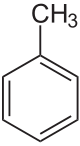
\includegraphics[width=0.1\linewidth]{gfx/e7_compound}
		\end{center}
	\caption[Aniline]{\label{e7_compound}}
	\end{figure}


	\begin{enumerate}
		\item Ethyl Acetate
		\item Toluene, refer to \autoref{e7_compound}
	\end{enumerate}


	% \begin{figure}[bth]
	% 	\begin{center}
	% 		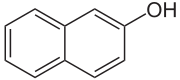
\includegraphics[width=0.4\linewidth]{gfx/e5_compound2}
	% 	\end{center}
	% \caption[2-Naphthol]{\label{e5_compound2}}
	% \end{figure}
\section {Apparatus/Setup}
	The setup is almost identical to that of the previous experiment. The only difference is that the still head in the previous experiment didn't have provision for providing extra surface area for condensation, whereas in this setup we have. It's called the fractionating column. Refer to \autoref{e6_setup} for details. The part labelled 3, is what's being referred to here.

\section{Theory}
	Fractional distillation is a method of separating constituents of a mixture which have a boiling point difference of less than $25 ^o C$. If the difference is greater than $25 ^o C$, then usual distillation suffices.
	\par
	The idea is the same as that of a simple distillation setup. The only difference, as mentioned earlier, is addition of a fractionating column. This is given very clearly in wikipedia and has been scarcely modified and stated here.
	\par
	The fractional distillation column is set up with the heat source at the bottom on the still pot. As the distance from the stillpot of the distillation column increases, a heat gradient is formed in the column where it is coolest at the top and hottest at the bottom. As the mixed vapour ascends through the temperature gradient, some of the vapour condenses and re-vaporizes. Each time the vapour condenses and vaporizes, the composition of the more volatile liquid in the vapour increases. This distills the vapour along the length of the column, and eventually the vapour is composed primarily of the more volatile liquid. The vapour condenses on the glass platforms, known as trays, inside the column, and runs back down into the liquid below, refluxing the distillate.

\section{Procedure}
	\begin{enumerate}
		\item The system was setup as shown in \autoref{e6_setup} with the fractionating column as described earlier
		\item The water circulator was turned on after submersing it in a large water bath
		\item The heating was initiated and temperature monitored to keep it in the 80-85 $^o C$ range
		\item The liquid took some time, but eventually started coming out in the collection flask
		\item When the process stopped, the collection flask was changed and the heating was increased gradually. Note that the temperature of the thermometer is likely to drop during this time as there are no vapours in contact with the thermometer at this stage
		\item This time the temperature was monitored to be in the 95-105 $^o C$ range
		\item The heating was first reduced when the volume dropped and the process was halted when the decrease was substantial
	\end{enumerate}


\section{Observations and Results}
	For Ethyl Acetate, the mantle was kept at 30 (there weren't any units on the mantle). The thermometer stabilized at $84 ^o C$.
	After the process completed, the mantle was kept at 50, and when the volume of the distillate dropped, it was dropped to 30 for Toluene. The thermometer stabilized at $100 ^o C$ for the same.

\section{Precaution}
	\begin{enumerate}
		\item The temperature of the thermometer would drop once one component has been separated. This doesn't mean the liquid is at that temperature, just that there isn't enough vapour in contact with the thermometer.
		\item Clean the thermometer holder in the apparatus, else there would be latency in reflection of temperature on the meter.
	\end{enumerate}
	Precautions given for the previous experiment must be taken here too.
	\begin{enumerate}
		\item Do not forget to use boiling chips, else unequal heat spread may result in explosive circumstances
		\item The water output should be facing upwards
		\item The condenser tube should be sufficiently slanted in the right direction to ensure the condensed liquid flows to the receiving flask and not the other way.
	\end{enumerate}

	
\section{Acknowledgements}
I thank Dr. R Vijaya Anand for his guidance during the experiment. I also acknowledge the contribution of my lab partners, Vivek, Prashansa and Srijit for performance of the same. I also thank our PhD guide for demonstrating the experiment and her assistance in general, with performance of the same.

	% \clearpage
	% \begin{figure}[bth]
	% 	\begin{center}
	% 		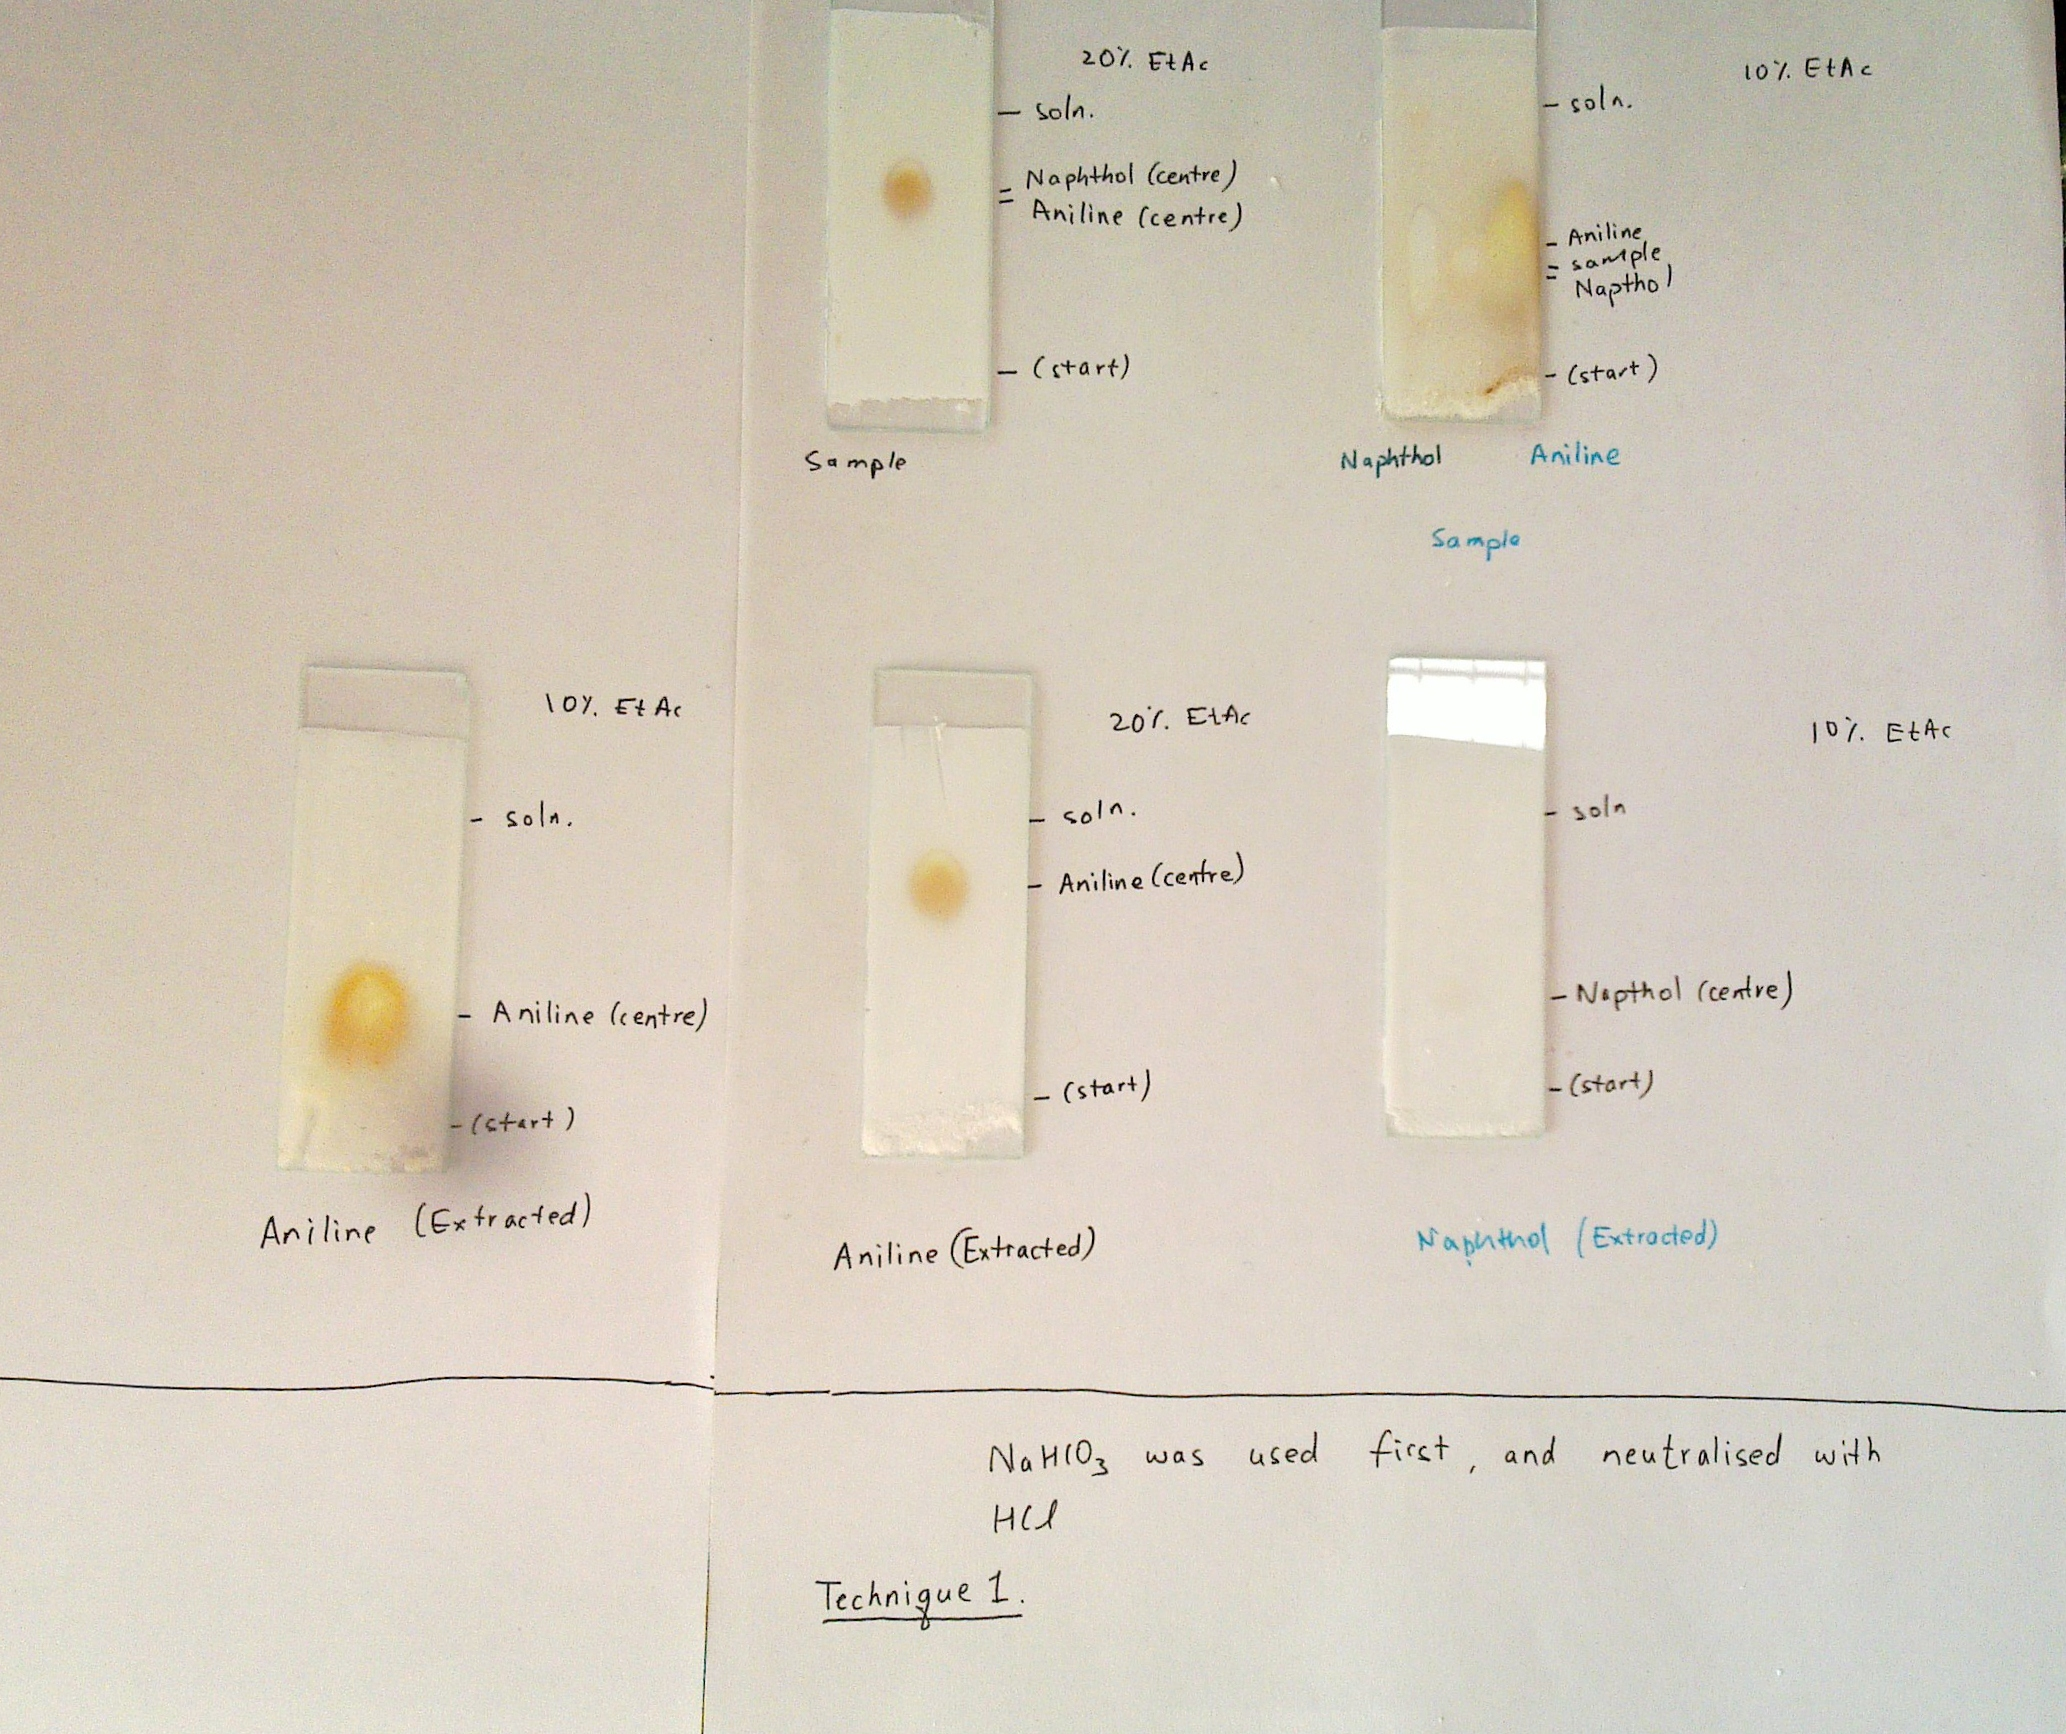
\includegraphics[width=1.5\linewidth]{gfx/e5_1}
	% 	\end{center}
	% \caption[TLCs Set 1]{\label{e5_1}}
	% \end{figure}

	% \begin{figure}[bth]
	% 	\begin{center}
	% 		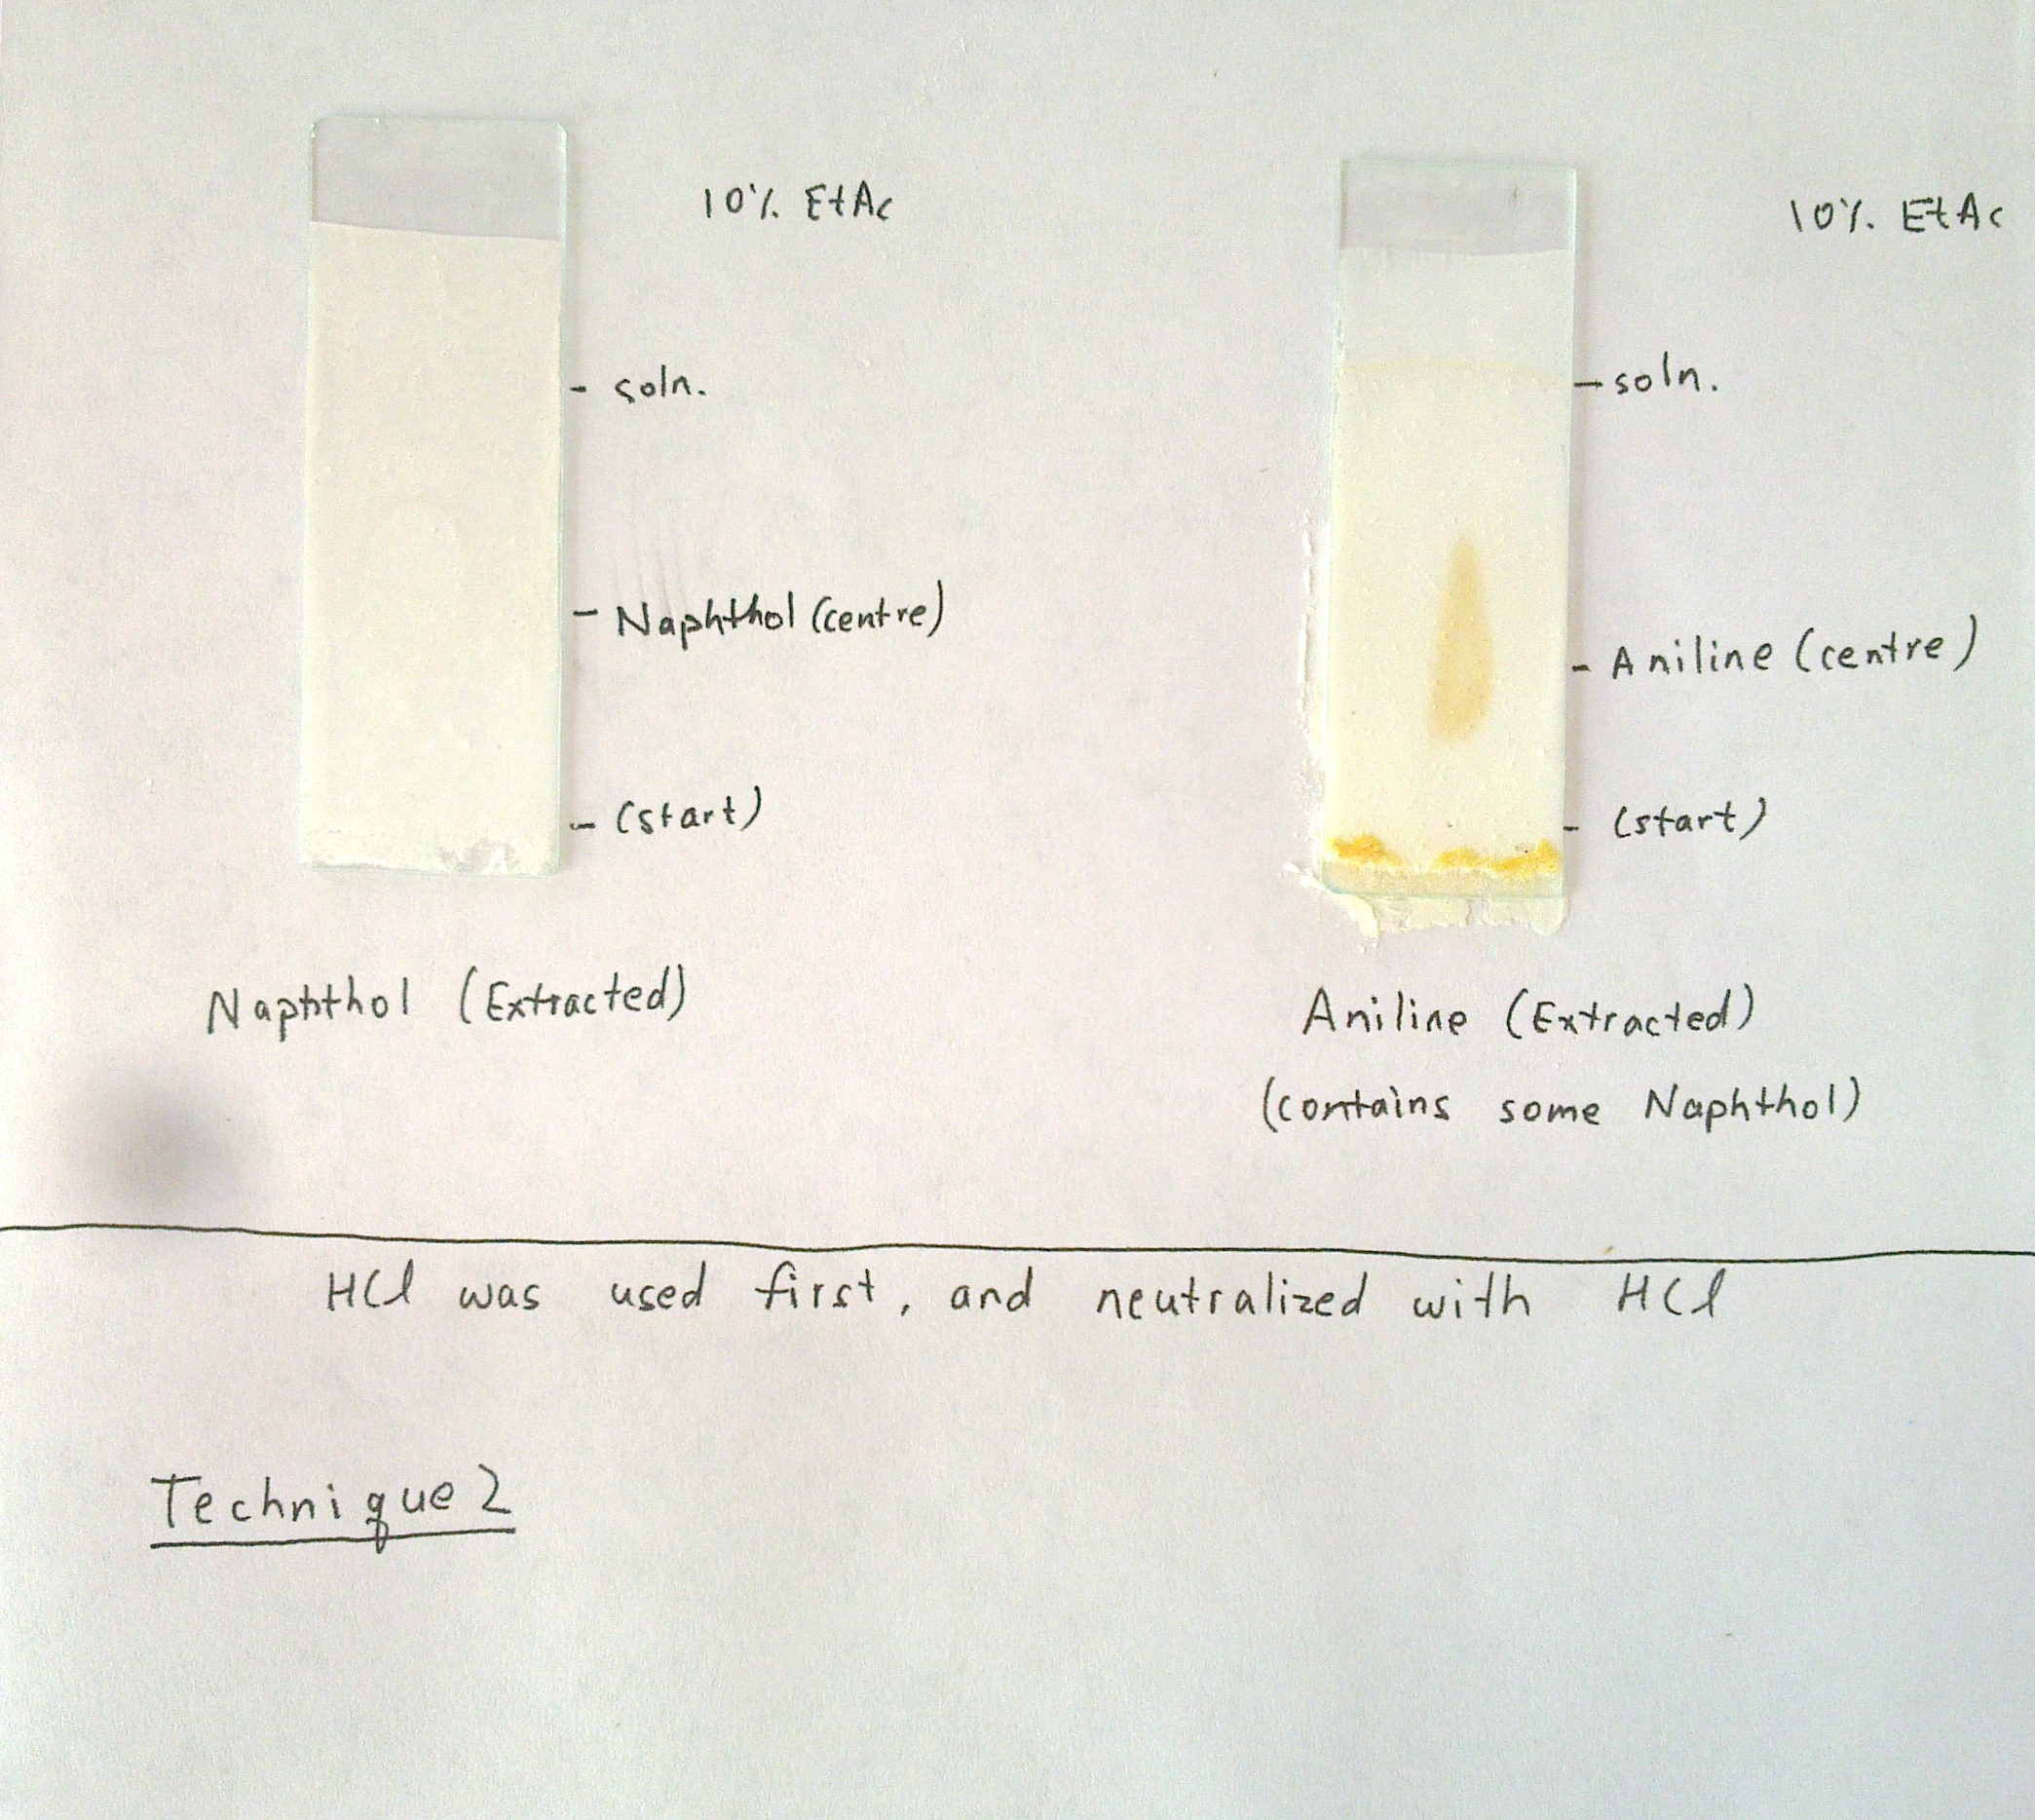
\includegraphics[width=1.0\linewidth]{gfx/e5_2}
	% 	\end{center}
	% \caption[TLCs Set 2]{\label{e5_2}}
	% \end{figure}